\documentclass[12pt]{article}
\usepackage{multicol}
\usepackage{cite}
\usepackage{listings}
\usepackage{tikz}
\usepackage[doublespacing]{setspace}

\usepackage{titlesec}
\newcommand{\sectionbreak}{\clearpage}
\usetikzlibrary{positioning}

\lstset{basicstyle=\ttfamily}

\author{Sammy Furr}
\title{The Development of a Collaborative Tool to Teach Debugging}
\date{\today}

\begin{document}

\begin{titlepage}
  \maketitle
\end{titlepage}

\begin{abstract}
  TODO: write an abstract
\end{abstract}

\tableofcontents
\pagebreak

\section{Introduction}
\subsection{Motivation}

Debugging is invaluable in writing and understanding code, yet it is
rarely formally taught\cite{doi:10.1080/08993400802114581}.  We
typically teach students programming structures, concepts, and
languages, but leave them to learn the tools they use to write code by
themselves.  This approach often works well---a programmer's choice of
tools is often \textit{very} personal and students figure out how to
configure an individualized workflow.  Perhaps because debuggers are
tools, students are often expected to learn them with minimal
guidance.  Unlike editors or reference guides however, effectively
using a debugger requires a set of high-level, platform agnostic,
teachable skills.  Teaching these skills is effective, and translates
into better, faster, debugging and
programming\cite{10.1145/3286960.3286970}\cite{10.1145/3361721.3361724}.

\subsubsection{The Value of Teaching Debugging}

There is an unfortunate lack of research specifically into the
efficacy of teaching debugging for computer science students, despite
a recent rise in the inclusion of debugging in ``computational
thinking'' curriculums\cite{10.1145/3361721.3361724}.  These
curriculums attempt to teach skills in computer science classes that
translate into other subject areas: the UK's computer science
curriculum considers debugging an essential ``transferable
skill''\cite{10.1145/2602484}.\par There seems to be confidence that
the problem-solving techniques used in debugging are widely
applicable, but of greater interest to computer science teachers is
whether teaching debugging directly benefits student programmers.
Michaeli and Romeike conducted a good, albeit somewhat small, study on
the efficacy of teaching a systematic debugging process to K12
students.  They found that students who have been taught a specific
debugging framework performed better in debugging tests and were more
confident in their own debugging skills\cite{10.1145/3361721.3361724}.
Their result is positive evidence towards the efficacy of teaching
debugging, though it doesn't include college or university
students.\par

As Michaeli and Romeike point out, there is a lack of research into
the value of teaching debugging in higher education.  None of the
research these authors found placed much focus on explicitly teaching
debugging.  Chmiel and Loui studied whether students who were provided
with debugging tools and frameworks performed better on tests or spent
less time on assignments than those who were
not\cite{10.1145/971300.971310}.  Though this research wasn't able to
find conclusive evidence towards better performance on tests or
assignments, it did find that students in the treatment group felt
more confident in their debugging abilities.  Unfortunately Chmiel and
Loui's study didn't involve extended explicit teaching of
debugging---use of the tools was voluntary, and variations in the
students' individual abilities made the data difficult to
evaluate.\par

Though there is a lack of higher-education research, the value of
teaching debugging is still demonstrable.  The research discussed all
finds that K-12 and college students alike commonly resort to sporadic
debugging techniques when beginning to learn.  Since this pattern of
behavior that explicitly teaching debugging corrects exists in college
as well as in K-12 students, it seems logical that the benefit of
explicitly teaching debugging to K-12 students should be realized
equally by their collegiate counterparts.\par

\subsubsection{Methods for Teaching Debugging}

Similarly to research on the value of teaching debugging, research
into how to best teach debugging is self-admittedly sparse.  Chan et
al. allow that ``in general research on how to improve debugging is
sporadic''---an observation that leads them to research a framework to
reduce the complexity of teaching
debugging\cite{10.1145/3286960.3286970}.  To organize their framework,
they split debugging knowledge into 5 categories: \textit{Domain},
\textit{System}, \textit{Procedural}, \textit{Strategic}, and
\textit{Experiential}.  They then review different debugging tools and
teaching aids---from those that involve writing code to games---and
map tools to the knowledge areas they seek to address.  After an
evaluation of a host of different tools, they claim to find a few
significant faults in current debugging teaching platforms. The
primary two which this project seeks to address are as follows:

\begin{enumerate}
\item A lack of back-tracing ability/coverage.
\item A lack of tools addressing system knowledge (an understanding of
  the program to be debugged).
\end{enumerate}

\subsubsection{The Value of Collaborative Programming}

TODO: find some basic research that backs up the claim that
collaborative/pair programming is worthwhile.

\subsubsection{Tools that Enable Collaborative Programming}

TODO: write about glitch, repl.it, etc.

\subsubsection{Collaborative Programming and Teaching Debugging}

Debuggers exist at an intersection of tools and skills similar to
programming languages themselves. By becoming familiar with a specific
debugger, students learn techniques and paradigms necessary to use all
debuggers effectively.
\pagebreak

\subsection{Project Components}

\tikzset{every picture/.style={line width=0.75pt}} %set default line width to 0.75pt
\tikzset{every picture/.style={baselineskip=1pt}}
\tikzset{every picture/.style={/utils/exec={\ttfamily}}}

\begin{figure}[h!]
  
  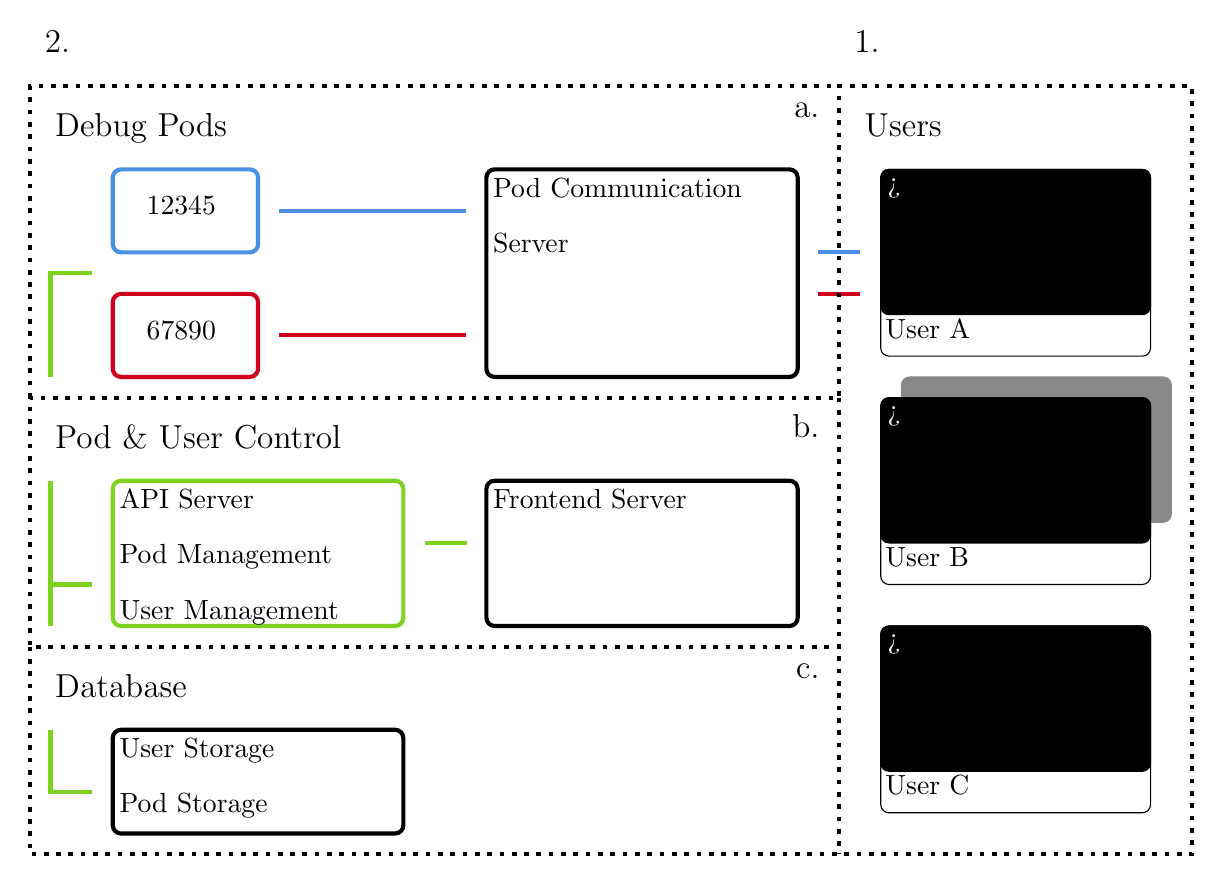
\begin{tikzpicture}[x=0.75pt,y=0.75pt,yscale=-1,xscale=1]
    % uncomment if require: \path (0,494); %set diagram left start at 0, and has height of 494

    % Straight Lines [id:da7736831842096191] 
    \draw [color={rgb, 255:red, 74; green, 144; blue, 226 }  ,draw opacity=1 ][line width=1.5]    (380,110) -- (400,110) ;
    % Shape: Rectangle [id:dp04619309000609384] 
    \draw  [color={rgb, 255:red, 136; green, 136; blue, 136 }  ,draw opacity=1 ][fill={rgb, 255:red, 136; green, 136; blue, 136 }  ,fill opacity=1 ] (420,174) .. controls (420,171.79) and (421.79,170) .. (424,170) -- (546,170) .. controls (548.21,170) and (550,171.79) .. (550,174) -- (550,236) .. controls (550,238.21) and (548.21,240) .. (546,240) -- (424,240) .. controls (421.79,240) and (420,238.21) .. (420,236) -- cycle ;
    % Shape: Rectangle [id:dp1228490870487785] 
    \draw   (410,74) .. controls (410,71.79) and (411.79,70) .. (414,70) -- (536,70) .. controls (538.21,70) and (540,71.79) .. (540,74) -- (540,156) .. controls (540,158.21) and (538.21,160) .. (536,160) -- (414,160) .. controls (411.79,160) and (410,158.21) .. (410,156) -- cycle ;
    % Shape: Rectangle [id:dp17147478083974088] 
    \draw  [color={rgb, 255:red, 0; green, 0; blue, 0 }  ,draw opacity=1 ][fill={rgb, 255:red, 0; green, 0; blue, 0 }  ,fill opacity=1 ] (410,74) .. controls (410,71.79) and (411.79,70) .. (414,70) -- (536,70) .. controls (538.21,70) and (540,71.79) .. (540,74) -- (540,136) .. controls (540,138.21) and (538.21,140) .. (536,140) -- (414,140) .. controls (411.79,140) and (410,138.21) .. (410,136) -- cycle ;
    % Shape: Rectangle [id:dp08735176678895862] 
    \draw   (410,184) .. controls (410,181.79) and (411.79,180) .. (414,180) -- (536,180) .. controls (538.21,180) and (540,181.79) .. (540,184) -- (540,266) .. controls (540,268.21) and (538.21,270) .. (536,270) -- (414,270) .. controls (411.79,270) and (410,268.21) .. (410,266) -- cycle ;
    % Shape: Rectangle [id:dp9595297060154465] 
    \draw  [color={rgb, 255:red, 0; green, 0; blue, 0 }  ,draw opacity=1 ][fill={rgb, 255:red, 0; green, 0; blue, 0 }  ,fill opacity=1 ] (410,184) .. controls (410,181.79) and (411.79,180) .. (414,180) -- (536,180) .. controls (538.21,180) and (540,181.79) .. (540,184) -- (540,246) .. controls (540,248.21) and (538.21,250) .. (536,250) -- (414,250) .. controls (411.79,250) and (410,248.21) .. (410,246) -- cycle ;
    % Shape: Rectangle [id:dp8231056072369544] 
    \draw   (410,294) .. controls (410,291.79) and (411.79,290) .. (414,290) -- (536,290) .. controls (538.21,290) and (540,291.79) .. (540,294) -- (540,376) .. controls (540,378.21) and (538.21,380) .. (536,380) -- (414,380) .. controls (411.79,380) and (410,378.21) .. (410,376) -- cycle ;
    % Shape: Rectangle [id:dp6367028620504607] 
    \draw  [color={rgb, 255:red, 0; green, 0; blue, 0 }  ,draw opacity=1 ][fill={rgb, 255:red, 0; green, 0; blue, 0 }  ,fill opacity=1 ] (410,294) .. controls (410,291.79) and (411.79,290) .. (414,290) -- (536,290) .. controls (538.21,290) and (540,291.79) .. (540,294) -- (540,356) .. controls (540,358.21) and (538.21,360) .. (536,360) -- (414,360) .. controls (411.79,360) and (410,358.21) .. (410,356) -- cycle ;
    % Shape: Rectangle [id:dp8426243961763082] 
    \draw  [color={rgb, 255:red, 74; green, 144; blue, 226 }  ,draw opacity=1 ][line width=1.5]  (40,74) .. controls (40,71.79) and (41.79,70) .. (44,70) -- (106,70) .. controls (108.21,70) and (110,71.79) .. (110,74) -- (110,106) .. controls (110,108.21) and (108.21,110) .. (106,110) -- (44,110) .. controls (41.79,110) and (40,108.21) .. (40,106) -- cycle ;
    % Shape: Rectangle [id:dp3822373593536188] 
    \draw  [color={rgb, 255:red, 208; green, 2; blue, 27 }  ,draw opacity=1 ][line width=1.5]  (40,134) .. controls (40,131.79) and (41.79,130) .. (44,130) -- (106,130) .. controls (108.21,130) and (110,131.79) .. (110,134) -- (110,166) .. controls (110,168.21) and (108.21,170) .. (106,170) -- (44,170) .. controls (41.79,170) and (40,168.21) .. (40,166) -- cycle ;
    % Straight Lines [id:da30880840083209404] 
    \draw [color={rgb, 255:red, 208; green, 2; blue, 27 }  ,draw opacity=1 ][line width=1.5]    (120,150) -- (210,150) ;
    % Shape: Rectangle [id:dp5669106087613988] 
    \draw  [line width=1.5]  (220,74) .. controls (220,71.79) and (221.79,70) .. (224,70) -- (366,70) .. controls (368.21,70) and (370,71.79) .. (370,74) -- (370,166) .. controls (370,168.21) and (368.21,170) .. (366,170) -- (224,170) .. controls (221.79,170) and (220,168.21) .. (220,166) -- cycle ;
    % Straight Lines [id:da24300582818436978] 
    \draw [color={rgb, 255:red, 74; green, 144; blue, 226 }  ,draw opacity=1 ][line width=1.5]    (120,90) -- (152.5,90) -- (210,90) ;
    % Straight Lines [id:da9215040164115669] 
    \draw [color={rgb, 255:red, 208; green, 2; blue, 27 }  ,draw opacity=1 ][line width=1.5]    (380,130) -- (400,130) ;
    % Shape: Rectangle [id:dp3848745776815077] 
    \draw  [color={rgb, 255:red, 126; green, 211; blue, 33 }  ,draw opacity=1 ][line width=1.5]  (40,224) .. controls (40,221.79) and (41.79,220) .. (44,220) -- (176,220) .. controls (178.21,220) and (180,221.79) .. (180,224) -- (180,286) .. controls (180,288.21) and (178.21,290) .. (176,290) -- (44,290) .. controls (41.79,290) and (40,288.21) .. (40,286) -- cycle ;
    % Shape: Rectangle [id:dp9909839356430334] 
    \draw  [line width=1.5]  (220,224) .. controls (220,221.79) and (221.79,220) .. (224,220) -- (366,220) .. controls (368.21,220) and (370,221.79) .. (370,224) -- (370,286) .. controls (370,288.21) and (368.21,290) .. (366,290) -- (224,290) .. controls (221.79,290) and (220,288.21) .. (220,286) -- cycle ;
    % Straight Lines [id:da7242957436529691] 
    \draw [color={rgb, 255:red, 126; green, 211; blue, 33 }  ,draw opacity=1 ][line width=1.5]    (190.5,250) -- (200,250) -- (210.5,250) ;
    % Straight Lines [id:da6155515815274885] 
    \draw [color={rgb, 255:red, 126; green, 211; blue, 33 }  ,draw opacity=1 ][line width=1.5]    (10,220) -- (10,290) -- (10,270) -- (30,270) ;
    % Shape: Rectangle [id:dp04289765101859899] 
    \draw  [line width=1.5]  (40,344) .. controls (40,341.79) and (41.79,340) .. (44,340) -- (176,340) .. controls (178.21,340) and (180,341.79) .. (180,344) -- (180,386) .. controls (180,388.21) and (178.21,390) .. (176,390) -- (44,390) .. controls (41.79,390) and (40,388.21) .. (40,386) -- cycle ;
    % Straight Lines [id:da912738070320213] 
    \draw [line width=1.5]  [dash pattern={on 1.69pt off 2.76pt}]  (0,300) -- (0,400) -- (560,400) -- (560,30) -- (390,30) -- (390,180) -- (0,180) -- (0,300) -- (290,300) -- (390,300) -- (390,400) ;
    % Straight Lines [id:da9646857023949835] 
    \draw [line width=1.5]  [dash pattern={on 1.69pt off 2.76pt}]  (390,180) -- (390,330) ;
    % Straight Lines [id:da36286215804614264] 
    \draw [line width=1.5]  [dash pattern={on 1.69pt off 2.76pt}]  (0,180) -- (0,30) -- (390,30) ;
    % Straight Lines [id:da5365951688341024] 
    \draw [color={rgb, 255:red, 126; green, 211; blue, 33 }  ,draw opacity=1 ][line width=1.5]    (10,340) -- (10,370) -- (30,370) ;
    % Straight Lines [id:da2808441683655002] 
    \draw [color={rgb, 255:red, 126; green, 211; blue, 33 }  ,draw opacity=1 ][line width=1.5]    (10,170) -- (10,120) -- (30,120) ;

    % Text Node
    \draw (411,141) node [anchor=north west][inner sep=0.75pt]   [align=left] {User A};
    % Text Node
    \draw (412,73) node [anchor=north west][inner sep=0.75pt]   [align=left] {\textcolor[rgb]{1,1,1}{>}};
    % Text Node
    \draw (411,251) node [anchor=north west][inner sep=0.75pt]   [align=left] {User B};
    % Text Node
    \draw (412,183) node [anchor=north west][inner sep=0.75pt]   [align=left] {\textcolor[rgb]{1,1,1}{>}};
    % Text Node
    \draw (411,361) node [anchor=north west][inner sep=0.75pt]   [align=left] {User C};
    % Text Node
    \draw (412,293) node [anchor=north west][inner sep=0.75pt]   [align=left] {\textcolor[rgb]{1,1,1}{>}};
    % Text Node
    \draw (51,82) node [anchor=north west][inner sep=0.75pt]   [align=left] {\begin{minipage}[lt]{31.110000000000003pt}\setlength\topsep{0pt}
        \begin{center}
          12345
        \end{center}

      \end{minipage}};
    % Text Node
    \draw (401,42) node [anchor=north west][inner sep=0.75pt]   [align=left] {{\large Users}};
    % Text Node
    \draw (11,42) node [anchor=north west][inner sep=0.75pt]   [align=left] {{\large Debug Pods}};
    % Text Node
    \draw (51,142) node [anchor=north west][inner sep=0.75pt]   [align=left] {\begin{minipage}[lt]{31.110000000000003pt}\setlength\topsep{0pt}
        \begin{center}
          67890
        \end{center}

      \end{minipage}};
    % Text Node
    \draw (222,73) node [anchor=north west][inner sep=0.75pt]   [align=left] {Pod Communication\\Server};
    % Text Node
    \draw (11,192) node [anchor=north west][inner sep=0.75pt]   [align=left] {{\large Pod \& User Control}};
    % Text Node
    \draw (42,223) node [anchor=north west][inner sep=0.75pt]   [align=left] {API Server\\Pod Management\\User Management};
    % Text Node
    \draw (222,223) node [anchor=north west][inner sep=0.75pt]   [align=left] {Frontend Server};
    % Text Node
    \draw (11,312) node [anchor=north west][inner sep=0.75pt]   [align=left] {{\large Database}};
    % Text Node
    \draw (42,343) node [anchor=north west][inner sep=0.75pt]   [align=left] {User Storage\\Pod Storage};
    % Text Node
    \draw (1,2) node [anchor=north west][inner sep=0.75pt]   [align=left] {\begin{minipage}[lt]{12.931356000000001pt}\setlength\topsep{0pt}
        \begin{flushright}
          {\large 2.}
        \end{flushright}

      \end{minipage}};
    % Text Node
    \draw (362,37) node [anchor=north west][inner sep=0.75pt]   [align=left] {\begin{minipage}[lt]{12.931356000000001pt}\setlength\topsep{0pt}
        \begin{flushright}
          {\large a.}
        \end{flushright}

      \end{minipage}};
    % Text Node
    \draw (391,2) node [anchor=north west][inner sep=0.75pt]   [align=left] {\begin{minipage}[lt]{12.931356000000001pt}\setlength\topsep{0pt}
        \begin{flushright}
          {\large 1.}
        \end{flushright}

      \end{minipage}};
    % Text Node
    \draw (362,187) node [anchor=north west][inner sep=0.75pt]   [align=left] {\begin{minipage}[lt]{12.931356000000001pt}\setlength\topsep{0pt}
        \begin{flushright}
          {\large b.}
        \end{flushright}

      \end{minipage}};
    % Text Node
    \draw (363,307) node [anchor=north west][inner sep=0.75pt]   [align=left] {\begin{minipage}[lt]{12.24pt}\setlength\topsep{0pt}
        \begin{flushright}
          {\large c.}
        \end{flushright}

      \end{minipage}};

  \end{tikzpicture}

  \caption{Overview of the Collaborative Debugger}
  \label{debugger:overview}
\end{figure}

The next sections give an overview of the various tools used to create
the collaborative debugger.  The debugger consists of:

\begin{enumerate}
\item A frontend web app built using React that presents a debugging
  interface to the end user (\ref{react}).
\item A distributed backend managed by Kubernetes (\ref{k8s}), split into three parts:
  \begin{enumerate}
  \item A pod for each debugging instance which runs the rr debugger
    (\ref{rr}).  These communicate directly with users through
    websockets (\ref{socketio}).
  \item Pods running a frontend server written in Node which works in
    tandem with an API server created using Flask (\ref{flask/node}).
    The API server manages creation and destruction of debug sessions,
    as well as authentication.
  \item A MongoDB database.
  \end{enumerate}
\end{enumerate}

\subsubsection{Kubernetes}\label{k8s}

Kubernetes is the defacto standard in container orchestration
software.  It provides a layer of abstraction on top of normal
containers, like those created by Docker.  By bundling one or more
closely linked containers into a ``pod'', Kubernetes is able to manage
deployment and re-deployment of applications running inside
containers.  It is trivial to create new pods, or to create multiple
pods running the same application as needed within a Kubernetes
cluster.  Kubernetes provides services to facilitate load balancing,
manage storage volumes,

\subsubsection{Mozilla's rr}\label{rr}

\paragraph{Overview}

rr is ``a lightweight tool for recording, replaying and debugging
execution of applications''.\cite{rr-repo} rr allows a programmer to
record the execution of a program on any compatible machine and replay
the execution later.  This enhances GDB's ability to ``time-travel''
when debugging, using commands such as \lstinline{reverse-continue}
and \lstinline{reverse-stepi}\cite{gdbman} to step backwards and
forwards through a program's execution.  Through a novel encapsulation
of the execution space, rr is able to deterministically record and
replay the execution of syscalls and other process behavior that
differs run-to-run.  This is invaluable when trying to debug behavior
that is not entirely dependent on the code being debugged.  A typical
workflow in rr consists of recording an inexplicable error, replaying
execution to find the area in which the error occurs, and then
narrowing in on the bug not by re-running the entire program, but by
progressing back and forth through execution in the problem area.

\paragraph{Limitations}

In comparison to solutions like PANDA\cite{10.1145/2843859.2843867}
that rely on capturing the entire state of of a virtual machine to
replay execution, rr records and replays faster, produces far smaller
files, and doesn't force execution inside of a
VM.\cite{DBLP:journals/corr/OCallahanJFHNP17} The tradeoff for these
benefits are two major system limitations: rr is only compatible with
the Linux kernel, and it's deterministic recording and replay relies
on a feature that is only found on modern \textit{Intel} x86 CPUs.
These limitations influenced the development of this project as a
webapp similar to existing tools for collaborative programming.
Luckily, the speed and size benefits of rr lend themselves well to
non-local execution.

\subsubsection{socket.io}\label{socketio}

\subsubsection{Flask and Node}\label{flask/node}

\subsubsection{React and Xterm.js}\label{react}

\subsection{Project Overview}

TODO: a brief overview linking aspects of the project to background
research discussed above.

\section{Design}

TODO: the big piece of writing, detailing components of the project,
the system as a whole, and motivations for design choices.

\section{Next Steps}

TODO: write about additional/necessary unimplemented features (ATM
this is looking like auth stuff, unless OAuth2 proves to be less of a
pain in the ass then when I've used it before in Javascript.  Maybe
some of the vis stuff as well, though I'd really like to get the
basics done here.)  Write about desire to actually do research and see
whether the tool helps students learn debugging.

\pagebreak
\bibliographystyle{acm}
\bibliography{sprojbib}{}
\end{document}
